\documentclass[11pt]{article}
\usepackage[top=0in, bottom=0.5in, left=1in, right=1in]{geometry}
\usepackage[T1]{fontenc}
\usepackage[polish]{babel}
\usepackage[utf8]{inputenc}
\usepackage{lmodern}
\selectlanguage{polish}
\usepackage{graphicx}
\begin{document}
\title{Laboratorium 1}
\author{Jan Seredyński}
\date{\today}
\maketitle

\section{Wstęp}
Zadaniem laboratorium było stworzenie programu, który mnoży kolejne liczby przez 2,
 a następnie umożliwia uruchomienia części benchmarkującej, która sprawdza jak długo
wykonywał się algorytm mnożenia lub seria takich algorytmów.

\section{Sposób wykonania}
Głównym celem zadania bylo wykonanie funkcji benchmarkującej do podanego algorytmu.\\
Dzięki zastosowaniu klas abstrakcyjnych i metod wirtualnych byłem w stanie klasę MyBenchmark, po której algorytm mnożenia dziedziczył wirtualną metodę wykonywania algorytmu, która włączała 'stoper' -> wykonywała algorytm -> 'zatrzymywała stoper'. To pozwoliło mi na zmierzenie czasu wykonywanych algorytmów w zależoći od ilości seri oraz liczb do obrobienia.

\section{Funkcje dodatkowe}
Program posiada funkcję generowania liczb losowych na podstawie czasu działania maszyny oraz zapisywanie i wczytaywanie liczb z plików.

\section{Benchmark}
Utworzyłem graf pokazujący jak zmieniał się czas wykonania algorytmu od liczby powtórzen.
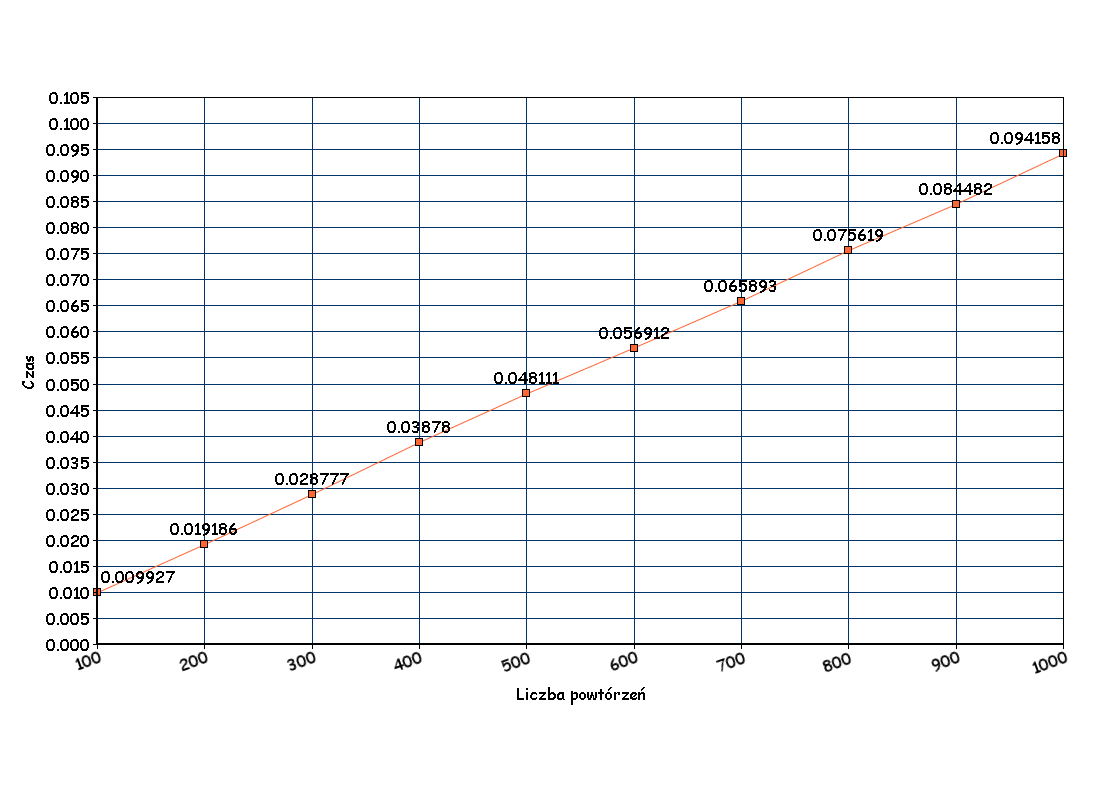
\includegraphics[width=4in]{blank.png} 


\section{Podsumowanie}
Zadanie zostało wykonane poprawnie, o czym świadczy wykres czasu od liczby powtórzen. Wykres odzwierciedla funkcję liniową, czyli czas i liczba powtórzen zmieniają sie proporcjonalnie, co należało wykazać w tym zadaniu.
\end{document}